یک تصویر $4\times 4 $ با ۱۶ پیکسل را در نظر بگیرید. هر پیکسل می‌تواند یکی از دو حالت سیاه (۱) یا سفید (۰) باشد (تصویر به صورت سیاه و سفید است). در این تصویر یک مربع $2 \times 2 $ وجود دارد که می‌خواهیم آن را تشخیص دهیم.

همان‌طور که گفته شد، تصویر سیاه و سفید است و مربع ایجاد می‌شود که ۴ پیکسل در کنار هم یک مقدار (۰ یا ۱) داشته باشند و دیگر پیکسل‌ها مقدار دیگری داشته باشند. با توجه به این موضوع می‌توان دریافت که در حالتی که بیشتر از یک مربع در تصویر ایجاد شود، مربع تشخیص داده نمی‌شود. نمونه‌های حضور مربع در زیر نمایش داده شده است:


\begin{figure}[h]
	\centering
	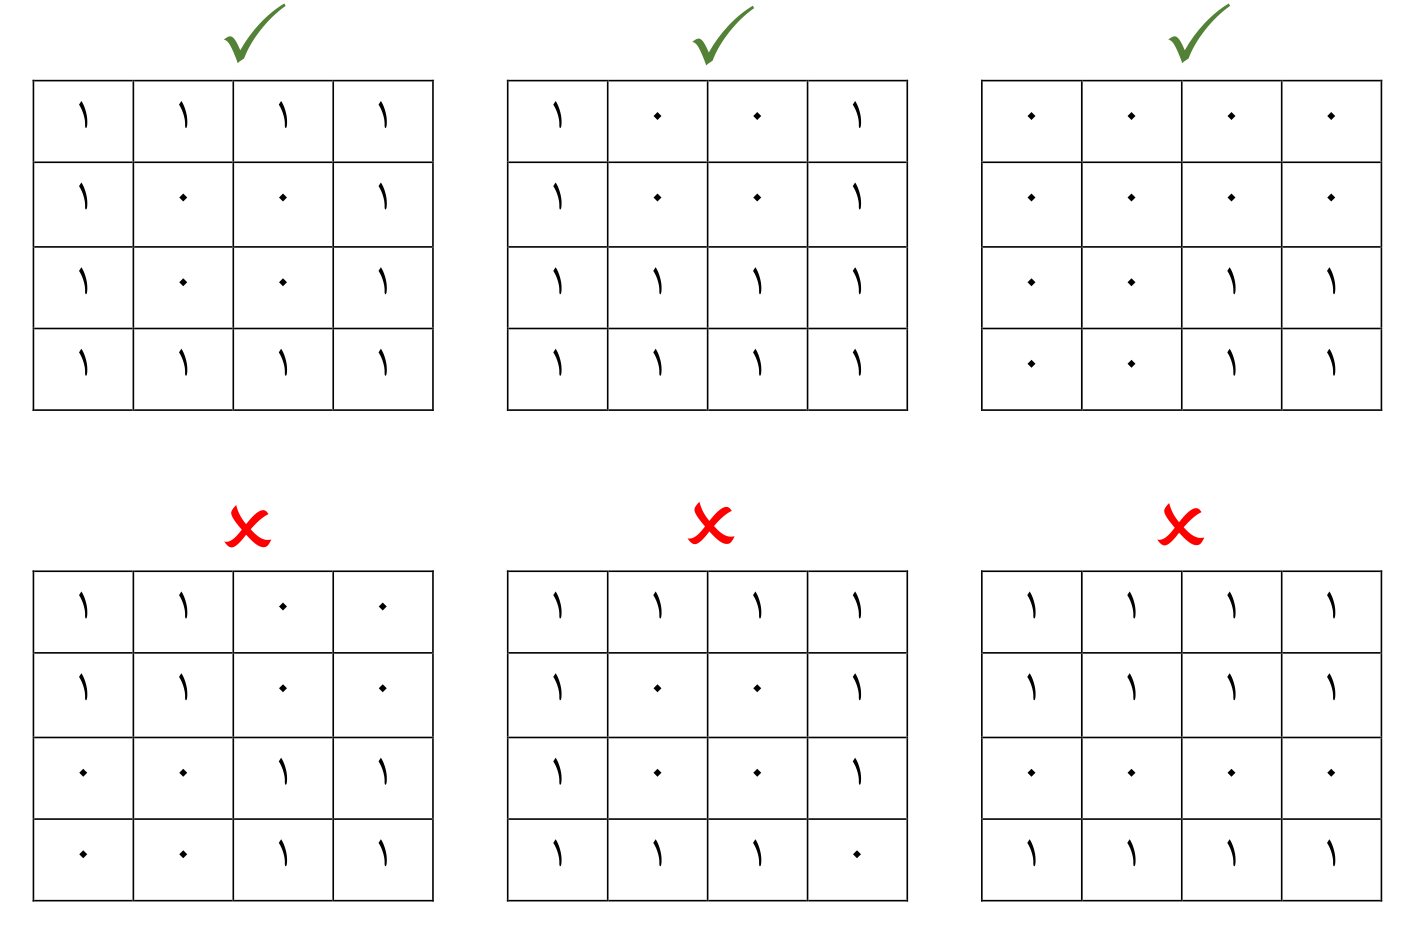
\includegraphics[width=0.9\textwidth]{fig/img4.png}
	\label{img4}
\end{figure}


تصویر از ۴ بلوک $2 \times 2 $  تشکیل شده است که هر کدام از این بلوک‌ها تنها می‌توانند یکی از چهار حالت
 زیر را داشته باشند.
 
 
 \begin{figure}[h]
 	\centering
 	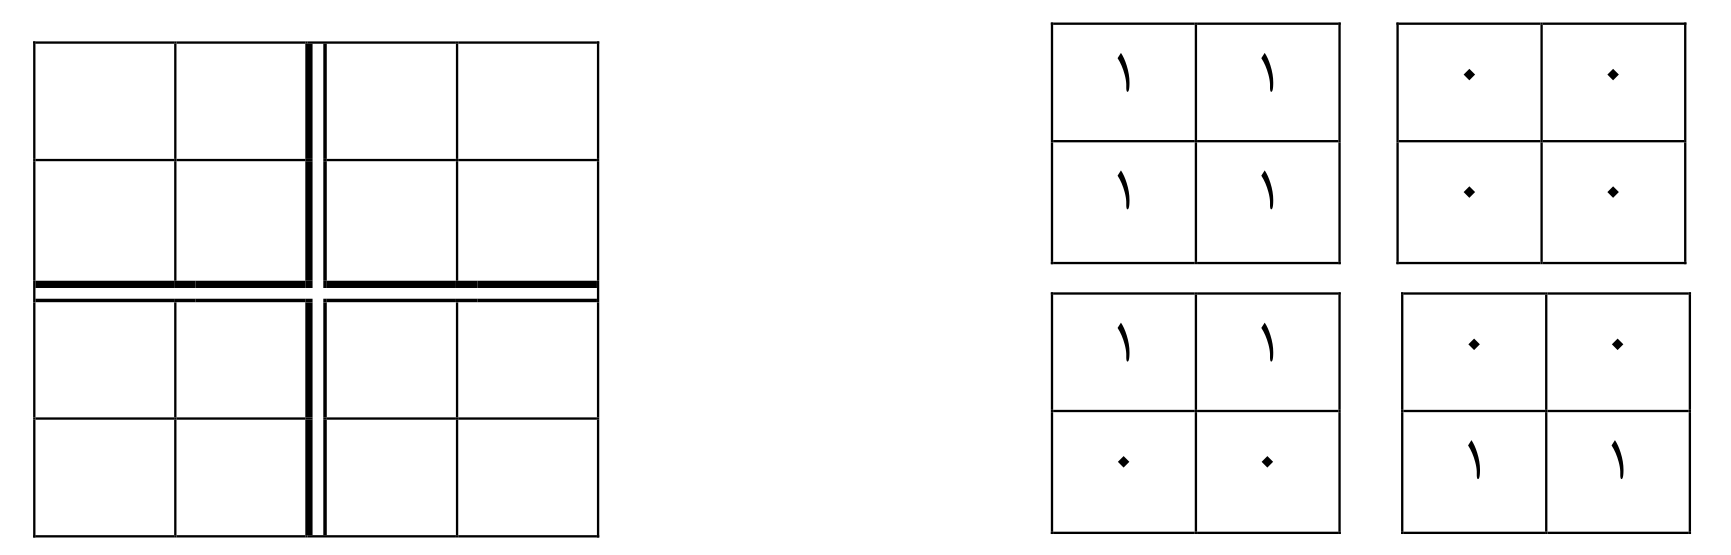
\includegraphics[width=0.9\textwidth]{fig/img5.png}
 	\label{img5}
 \end{figure}
 
 با توجه به توضیحات داده شده مداری طراحی کنید که حالات موجود در تصویر را دریافت کند بتواند مربع تولید شده در تصویر را تشخیص دهد. در صورت وجود یک مربع مقدار یک در خروجی ایجاد کند و در غیر این صورت مقدار صفر تولید کند.
 
 برای این کار مراحل زیر را انجام داده و گزارش دهید:
 
 \begin{enumerate}
 	\item ابتدا جدول صحت مدار مورد نظر را بنویسید.
 	\item تابع بولی به دست آمده از جدول صحت را بنویسید (بدون ساده‌سازی).
 	\item با استفاده از جدول کارنو تابع را ساده کنید.
 	\item مدار متناظر با تابع ساده شده را رسم کنید.
 \end{enumerate}